\documentclass[../sparc.tex]{subfiles}
\graphicspath{{\subfix{../images/}}}
\begin{document}

%%%%%%%%%%%%%%%%%%%%%%%%%%%%%%%%%%%%%%%%%%%%%%%%%%%%%%%%%%%%%%%%%%%%%%%%%%%%%%%%
\section{Аналогово-цифровое преобразование}

Чтобы не терялась нить повествования, в главе ``Использование потенциометра''
стоило умолчать о том, как Arduino проводит преобразование напряжения с
аналогового порта в дискретное значение от 0 до 1023. Задавшись вопросом -- ``А
почему именно 1023?'', мы сможем познакомиться с такой интересной штукой как
АЦП. \emph{Аналого-Цифровой Преобразователь} (АЦП) - это устройство, которое и
проводит преобразование.

Преобразование проходит в три этапа:
\begin{enumerate}
\item \emph{Дискретизация.} Выбираются значения из исходного аналогового сигнала через
  равные временные промежутки (\ref{fig:discretization}.)

  \begin{figure}[h]
    \caption{Дискретизация.}
    \label{fig:discretization}
    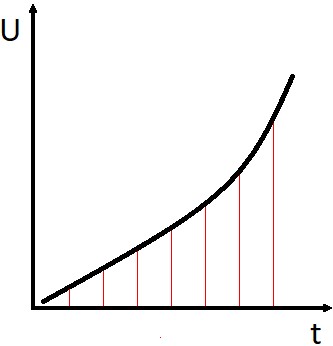
\includegraphics[width=8cm]{discretization}
    \centering
  \end{figure}

  Характеристика, отражающая эти временные промежутки, называется частота
  дискретизации.
\item \emph{Квантование.} Полученные значения заменяются ближайшим значением из
  набора фиксированных величин -- \emph{уровней квантования}
  (\ref{fig:quantization}.)

  \begin{figure}[h]
    \caption{Квантование.}
    \label{fig:quantization}
    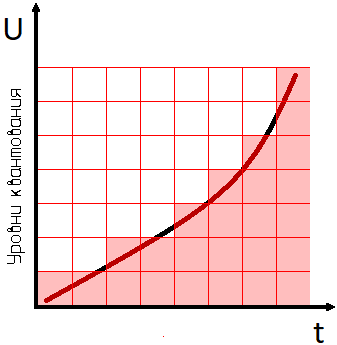
\includegraphics[width=8cm]{quantization}
    \centering
  \end{figure}

\item \emph{Кодирование.} Квантованным значениям присваивается цифровой код
  (\ref{fig:coding}.)

  \begin{figure}[h]
    \caption{Кодирование.}
    \label{fig:coding}
    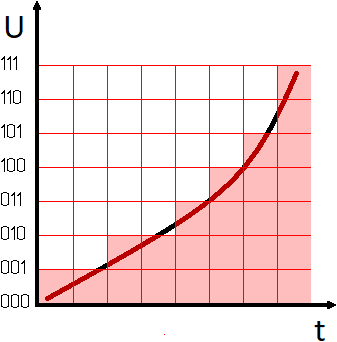
\includegraphics[width=8cm]{coding}
    \centering
  \end{figure}

  Чем выше частота дискретизации и чем больше уровней квантования, тем точнее
  преобразование.

\end{enumerate}

Одной из характеристик АЦП является \emph{разрядность}. Она определяет
количество значений, которое может выдать АЦП. Посмотрим на последний график:
для кодирования значений используется три бита, значит АЦП, описываемый таким
графиком, имеет, соответственно, разрядность 3 бита. То есть $ 2^3 = 8 $, что
равно количеству уровней квантования.

Вот и ответ на поставленный вопрос. АЦП Arduino 10-ти разрядный, $2^{10} = 1024$.
Именно столько значений АЦП Arduino может выдать.

Ещё есть такое устройство как ЦАП - \emph{Цифро-Аналоговый Преобразователь},
который, как нетрудно догадаться, выполняет функцию, обратную функции АЦП -
преобразует цифровой сигнал в аналоговый. Область применения ЦАП и АЦП
достаточно широка: в звуковых и видео- картах, в мониторах, в различной
акустической аппаратуре, в измерительных приборах, и многих других видах
техники.

Стоит упомянуть про 8-битную музыку в древних игровых консолях. Её название
отражает разрядность ЦАП звуковых чипов тех консолей -- 8 бит. Именно такой ЦАП
позволял выдавать тот самый резковатый, хлопающий и шипящий звук.

\end{document}
